\renewcommand{\thechapter}{\arabic{chapter}}
\setcounter{chapter}{0}

\chapter{La peau et ses lésions}
\label{chap:chapter_1}
\chapterintro
Comme introduction à ces travaux, ce premier chapitre permet d'apporter une description de l'organe majeure de cette étude : la peau. Il a donc pour but de poser les bases et ainsi permettre une compréhension sur sa physiologie, son fonctionnement et ses rôles. Par ces quelques pages nous décrivons pas à pas différents aspects. Dans un premier temps, une explication de ses principales couches et composantes est faite, et ceci par profondeur croissante. Ensuite, une partie est consacrée à la présentation de quelques unes de ses principales lésions puisque étant le sujet principal de cette étude. Par ailleurs, ces pages sont l'occasion d'aborder une première fois le Lentigo, pathologie centrale de cette étude, et tout particulièrement ses formes malignes : le Lentigo Maligna et le Lentigo Maligna Melanoma.\par
\newpage

\section{Présentation, composition et fonctions}
Avant d’aborder les lésions pouvant affecter cet organe, nous allons introduire de manière synthétique sa composition et son fonctionnement. Nous étudierons chaque couche évoquée par ordre de profondeur croissante.\par

\subsection{Présentation}
Le terme "peau" caractérise dans son sens le plus global, l’enveloppe externe propre aux vertébrés. Présente chez l’homme, elle est l’un de ses organes majeurs mais également l’un des plus lourds : chez un individu adulte d’un poids de \SI{70}{\kilo\gram}, elle représente une surface plane d’environ \SI{2}{\metre\squared}, soit une masse estimée à \SI{5}{\kilo\gram} \cite{McGrath2010}. Son épaisseur diffère selon la zone du corps étudiée : de \SI{0,5}{\milli\metre} au niveau de zones fines telles que les paupières, à \SI{5}{\milli\metre} sur des zones plus épaisses telles que le haut du dos. Cet organe souvent méconnu, voire oublié par la plupart d’entre nous, assure pourtant des fonctionnalités multiples : 
\begin{itemize}
\item La protection contre le monde extérieur
\item La limitation de la perte d’eau
\item La thermorégulation
\item L’appréhension physique de notre monde
\item \ldots
\end{itemize}\par
La dermatologie, branche médicale vouée à l’étude de la peau, nous permet de mieux comprendre sa composition, son fonctionnement, ses vulnérabilités et permet d’apporter conseils, préventions et traitements dans le cas de certaines pathologies.\par
Cette barrière se décompose en diverses couches fondamentales : l’épiderme, la membrane basale, le derme et l’hypoderme, dont la représentation est visible au travers de la \Cref{fig:illustration_skin_kholoski}.\par
\begin{figure}[H]
    \centering
    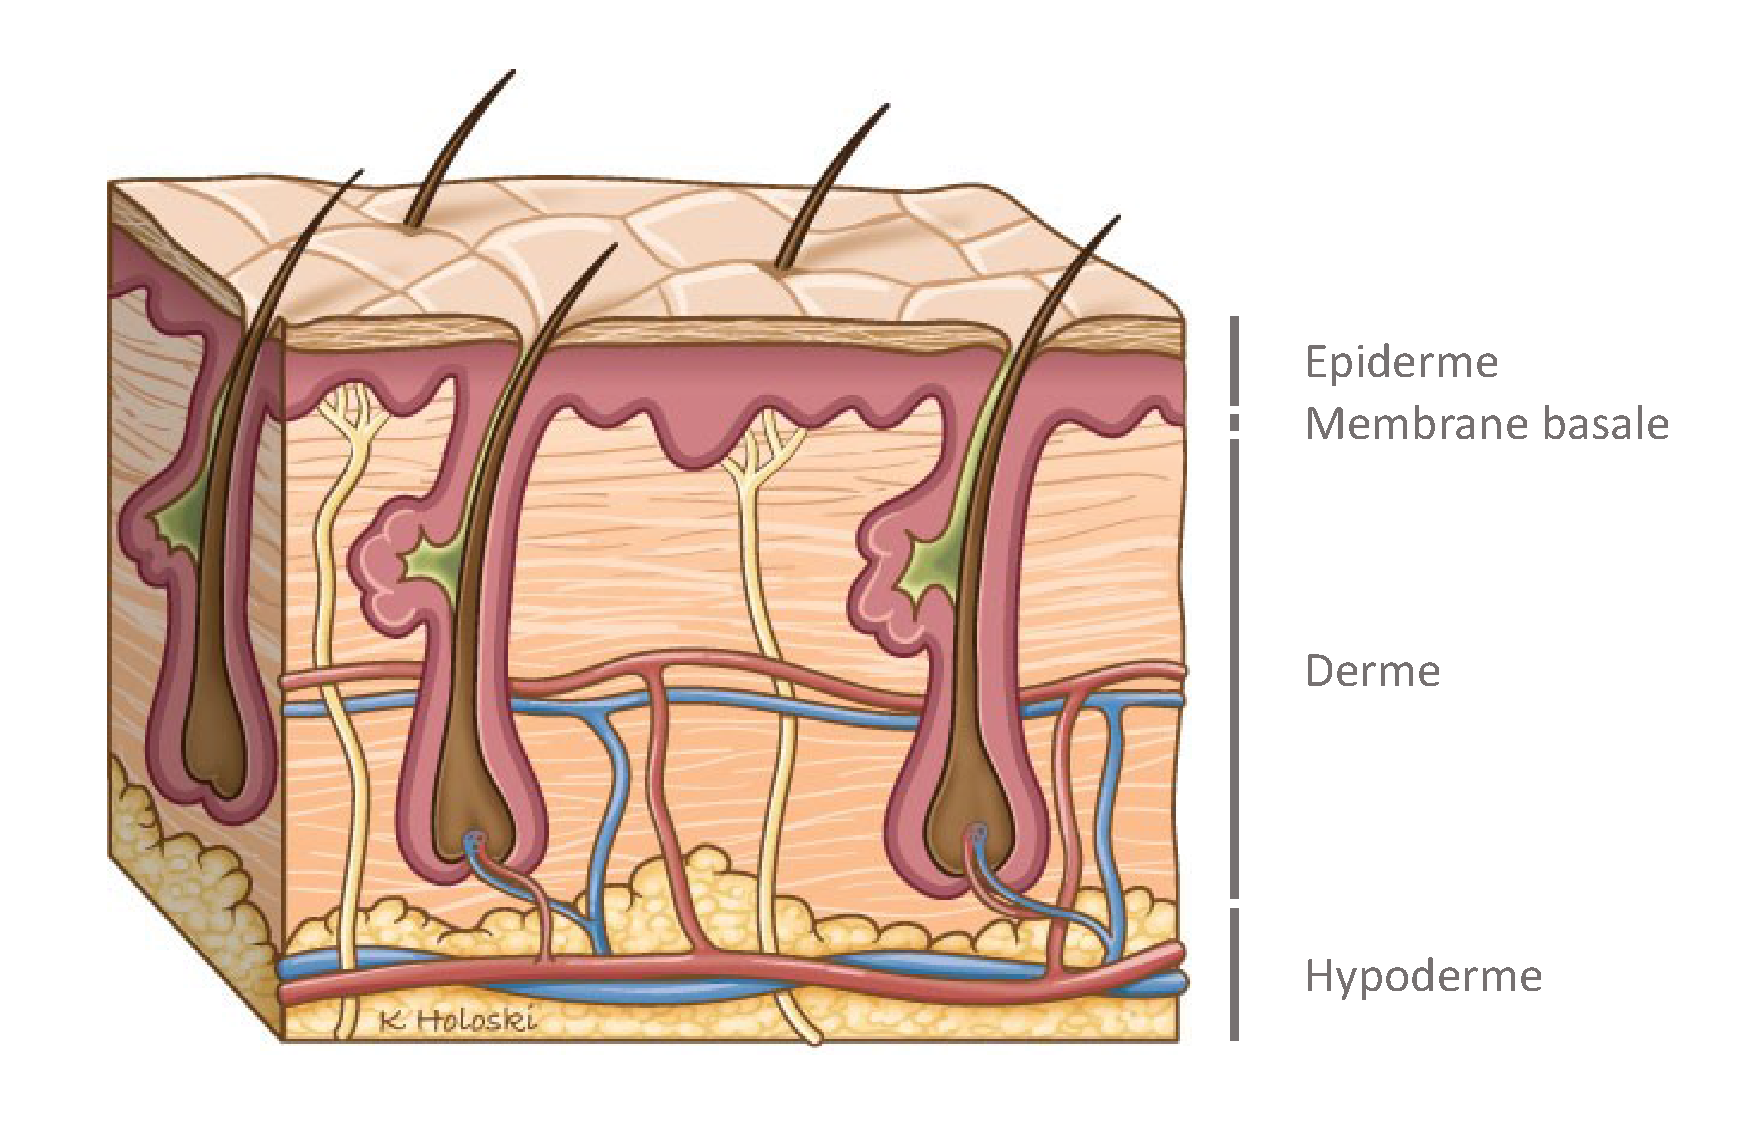
\includegraphics[width=0.6\linewidth]{contents/chapter_1/resources/illustration_skin_kholoski.png}
    \caption{Illustration macroscopique de la peau \textsuperscript{\ref{footnote:illustration_skin_kholoski}}. Les diverses couches composant la peau y sont réprésentées : l'épiderme, le derme et l'hypoderme.}
    \label{fig:illustration_skin_kholoski}
\end{figure}
\addtocounter{footnote}{1}
\footnotetext[\thefootnote]{Image source : Dessin par \href{http://kholoski.com/}{Kellie Holoski} – Illustrateur médical. \label{footnote:illustration_skin_kholoski}}
\clearpage

\subsection{Épiderme}
L’épiderme correspond à la couche superficielle de notre peau et mesure entre \SI{0,01}{\milli\metre} et \SI{0,1}{\milli\metre} d’épaisseur \cite{Sandby-Moller2003}. Un aperçu des différents types de cellules la composant peut être visible sur la \Cref{fig:illustration_epidermis_kholoski}, parmi lesquelles :
\begin{itemize}
\item Kératinocytes : 90 \% des cellules, rôle de protection
\item Cellules de Langerhans : cellules immunitaires
\item Cellules de Merkel : cellules sensitives
\item Mélanocytes : cellules de protection contre les \gls{uv}.
\end{itemize}\par

 \begin{figure}[H]
    \centering
    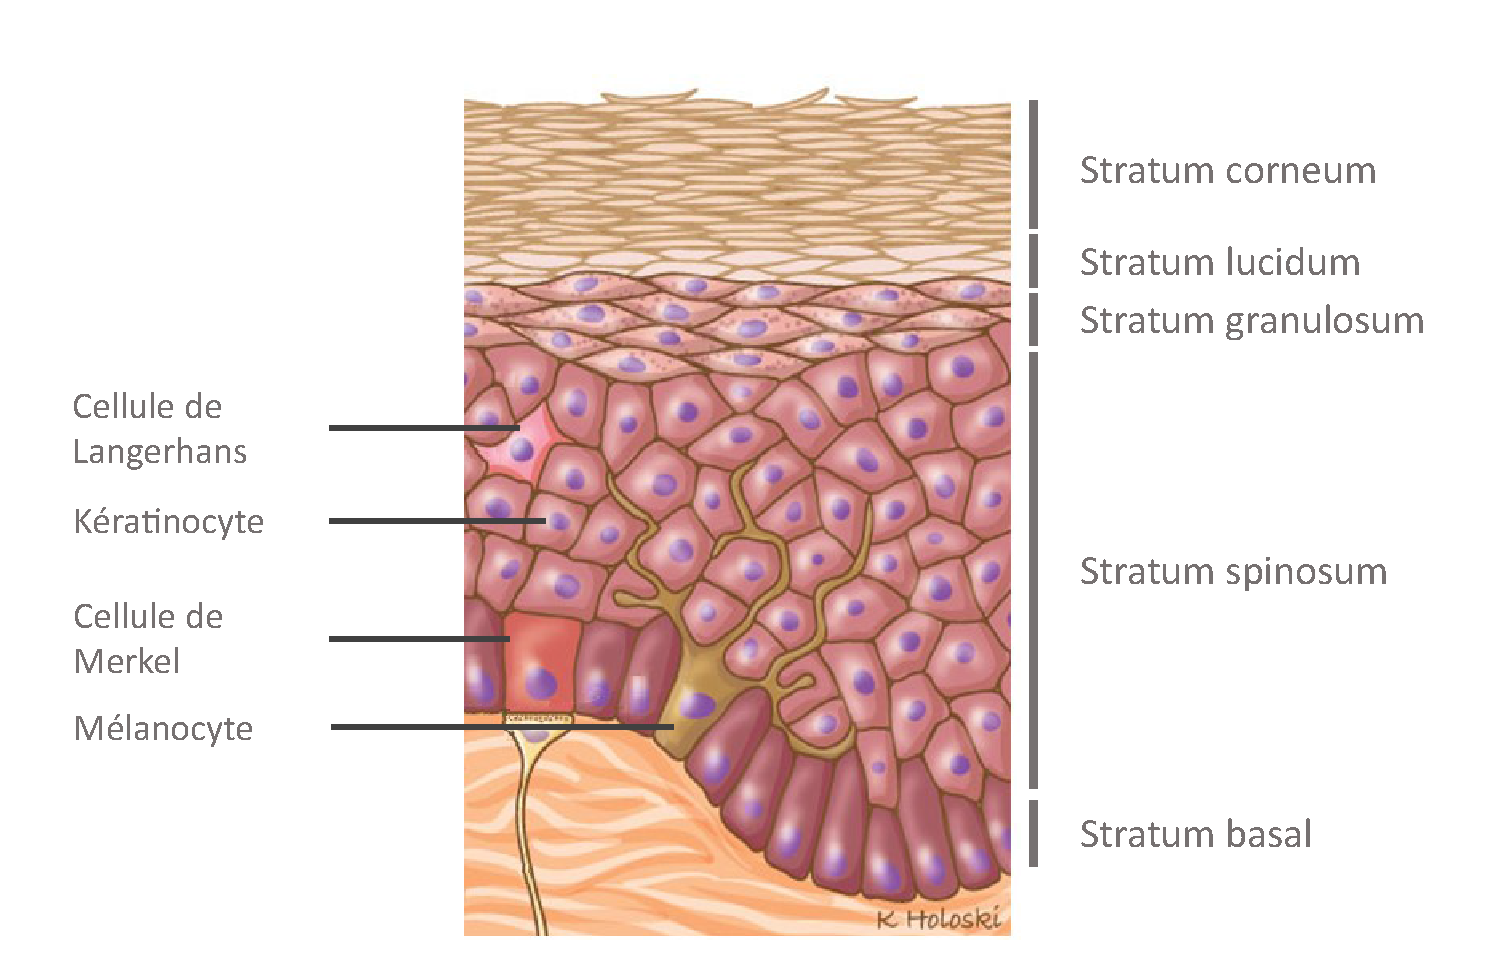
\includegraphics[width=0.7\linewidth]{contents/chapter_1/resources/illustration_epidermis_kholoski.png}
    \caption{Illustration des diverses couches composant l'épiderme (formée par un processus de différenciation) ainsi que ses divers composés cellulaires \textsuperscript{\ref{footnote:illustration_epidermis_kholoski}}.}
    \label{fig:illustration_epidermis_kholoski}
\end{figure}\par

\addtocounter{footnote}{1}
\footnotetext[\thefootnote]{Image source : Dessin par \href{http://kholoski.com/}{Kellie Holoski} – Illustrateur médical. \label{footnote:illustration_epidermis_kholoski}}

Son processus de différenciation des cellules est l’une de ses caractéristiques essentielles. Les kératinocytes, sa principale composante, migrent de la couche inférieure à la couche supérieure en subissant différentes modifications chimiques conduisant à la perte de leur noyau et à la mort de ces cellules. Ce processus porte le nom de kératinisation, et se subdivise en sous couches aux propriétés variées, respectivement par profondeur croissante : Cornée (Stratum corneum), Transition (Stratum lucidum), Granuleuse (Stratum granulosum), Epineuse (Stratum spinosum), Basale (Stratum basale). Ces différentes couches peuvent être observées sur la \Cref{fig:illustration_epidermis_kholoski}. En fin de parcours, ces cellules perdent leur cohésion dans un processus de desquamation conduisant la peau à se renouveler.\par\clearpage

\subsection{Jonction dermo-épidermique}
La \gls{dej}, ou encore membrane basale, se situe à la jonction de l’épiderme et du derme, et peut être observée par microscopie optique ou électronique selon l’épaisseur de cette dernière. Son épaisseur, variable selon la zone considérée, est estimée entre \SI{60}{\nano\metre} et \SI{300}{\nano\metre}. 
Cette membrane est scindée en 2 parties :
\begin{itemize}
\item La lame basale (lamina basalis), divisée en deux couches : Lamina Lucida et Lamina Densa
\item La lame réticulaire ou zone fibrillaire (lamina reticularis ou fibroreticularis).
\end{itemize}\par
\begin{figure}[H]
    \centering
    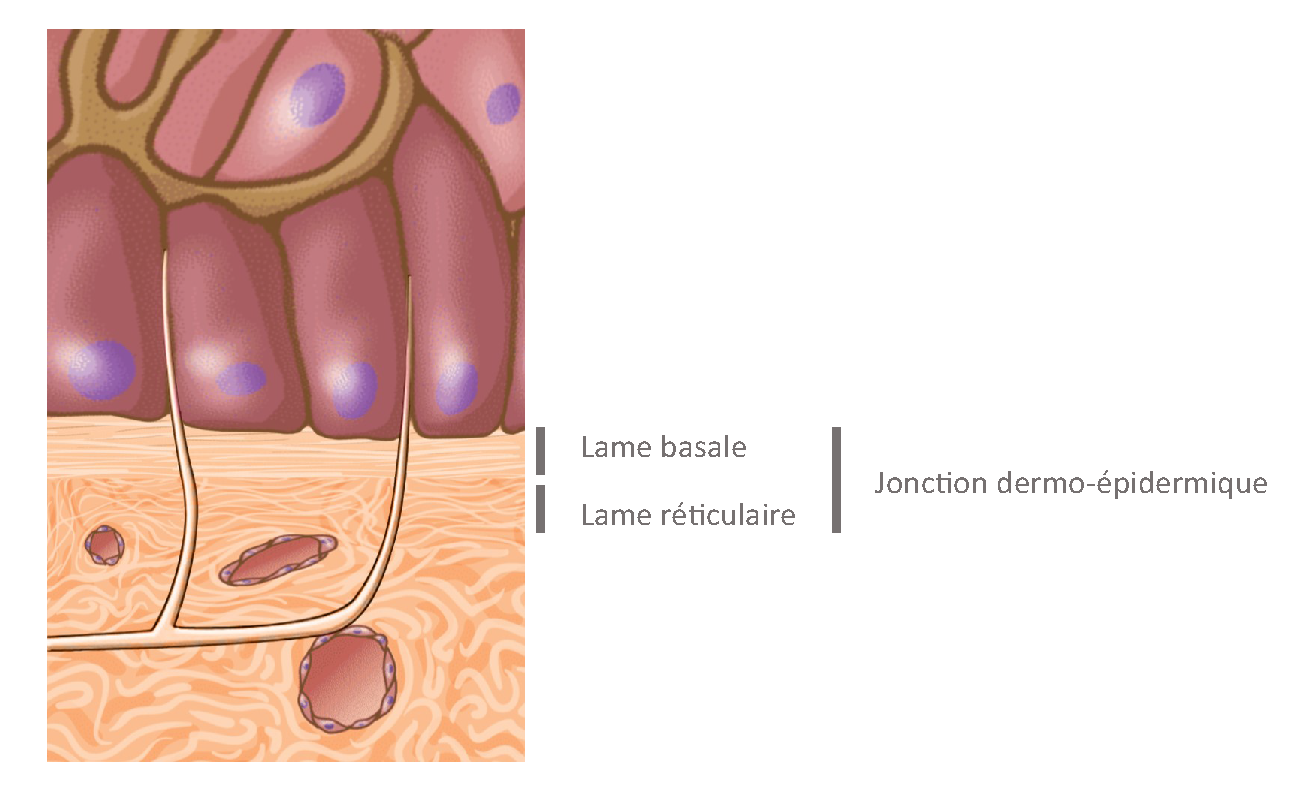
\includegraphics[width=\linewidth]{contents/chapter_1/resources/illustration_basal_basement.pdf}
    \caption{Illustration de la jonction dermo-épidermique \textsuperscript{\ref{footnote:illustration_basal_basement}}. Cette jonction dont le rôle est d'assurer une cohésion entre l'épiderme et le derme peut être subdivisée en deux sous couches : la lame basale et réticulaire. }
    \label{fig:illustration_basal_basement}
\end{figure}\par

\addtocounter{footnote}{1}
\footnotetext[\thefootnote]{Image source : Principles of Anatomy and Physiology – John Wiley \& Sons. \label{footnote:illustration_basal_basement}}

Il s’agit d’une zone fibreuse, composée de laminine, de collagène de type III / IV / VI lui conférant entre autres des propriétés de résistance mécanique, voire élastiques. Ces fibres lui permettent d’assurer une cohésion entre épiderme et derme au travers de points d’ancrage. Sa seconde fonction essentielle est au travers d’un mécanisme de régulation des échanges moléculaires, permettant d’assurer la nutrition des cellules de base de l’épiderme. Pour finir, elle possède un rôle de ré épidermisation fondamentale lors de la cicatrisation.\par
\clearpage

\subsection{Derme}
Le derme est une couche d’une épaisseur estimée comprise entre \SI{0,5}{\milli\metre} et \SI{5}{\milli\metre}, composée majoritairement de collagène à hauteur de 80 \% (sur la matières sèche), et de fibres élastiques \cite{McGrath2010}. Cette couche est traversée par de nombreux éléments dont : 

\begin{itemize}
\item Des vaisseaux sanguins, qui apportent nutriments
\item Des vaisseaux lymphatiques, qui assurent une fonction immunitaire.
\end{itemize}\par

En outre, cette strate contribue de manière essentielle à des aspects de résistance et contrainte mécanique de la peau, ainsi qu’aux mécanismes de thermorégulation et de cicatrisation de cette dernière. Enfin, cette couche tient un rôle essentiel dans la perception sensorielle (somesthésie) assurant d’une part des propriétés liées à la pression (mécanorécepteurs) mais également liées à la chaleur (thermorécepteurs). Outre ces fonctions, on lui attribue également un rôle nutritif important de par son irrigation sanguine.\par
La littérature identifie deux parties majeures au sein du derme,t visibles en \Cref{fig:illustration_dermis_kholoski}. Nous retrouvons:
\begin{itemize}
\item Le derme Papillaire (Papillary dermis), permettant essentiellement la thermorégulation
\item Le derme Réticulaire (Reticular dermis), assurant la plupart des fonctions mécaniques.
\end{itemize}\par

\begin{figure}[H]
    \centering
    \includegraphics[width=\linewidth]{contents/chapter_1/resources/illustration_dermis_kholoski.pdf}
    \caption{Illustration de représentation du derme \textsuperscript{\ref{footnote:illustration_dermis_kholoski}}. Le derme est subdivisée en deux couches aux propriétés distinctes: le derme papillaire et réticulaire.}
    \label{fig:illustration_dermis_kholoski}
\end{figure}\par

\addtocounter{footnote}{1}
\footnotetext[\thefootnote]{Image source : Dessin par \href{http://kholoski.com/}{Kellie Holoski} – Illustrateur médical. \label{footnote:illustration_dermis_kholoski}}
\clearpage

\subsection{Hypoderme}
L’hypoderme, également appelée couche sous cutanée, est un tissu présent sous le derme composé essentiellement de graisses (adipocytes, cellules spécialisées dans le stockage de graisses). Son épaisseur est extrêmement variable de \SI{0,1}{\centi\metre} à \SI[parse-numbers = false]{plusieurs}{\centi\metre}, selon :
\begin{itemize}
\item La zone considérée
\item L’âge du patient
\item L’alimentation
\item Les prédispositions génétiques.
\end{itemize}\par

Cette couche de tissu assure diverses fonctions, dont :
\begin{itemize}
\item Le passage des vaisseaux sanguins et lymphatiques, ainsi que celui des nerfs jusqu’au derme
\item L’interface entre les structures sous cutanées et la peau.
\end{itemize}\par

\subsection{Types de peau}
Il est nécessaire afin de bien aborder ce sujet et ses problématiques, d’être conscient des variations inter individus. Pour répondre partiellement à ces variations, Fitzpatrick a établi une classification des profils type de peau, visant à caractériser leur réaction suite à l’exposition au soleil. Ce travail a également permis de créer une association entre profil type et couleur de peau avant et après exposition au soleil \cite{Fitzpatrick1988}. 
\begin{figure}[H]
    \centering
    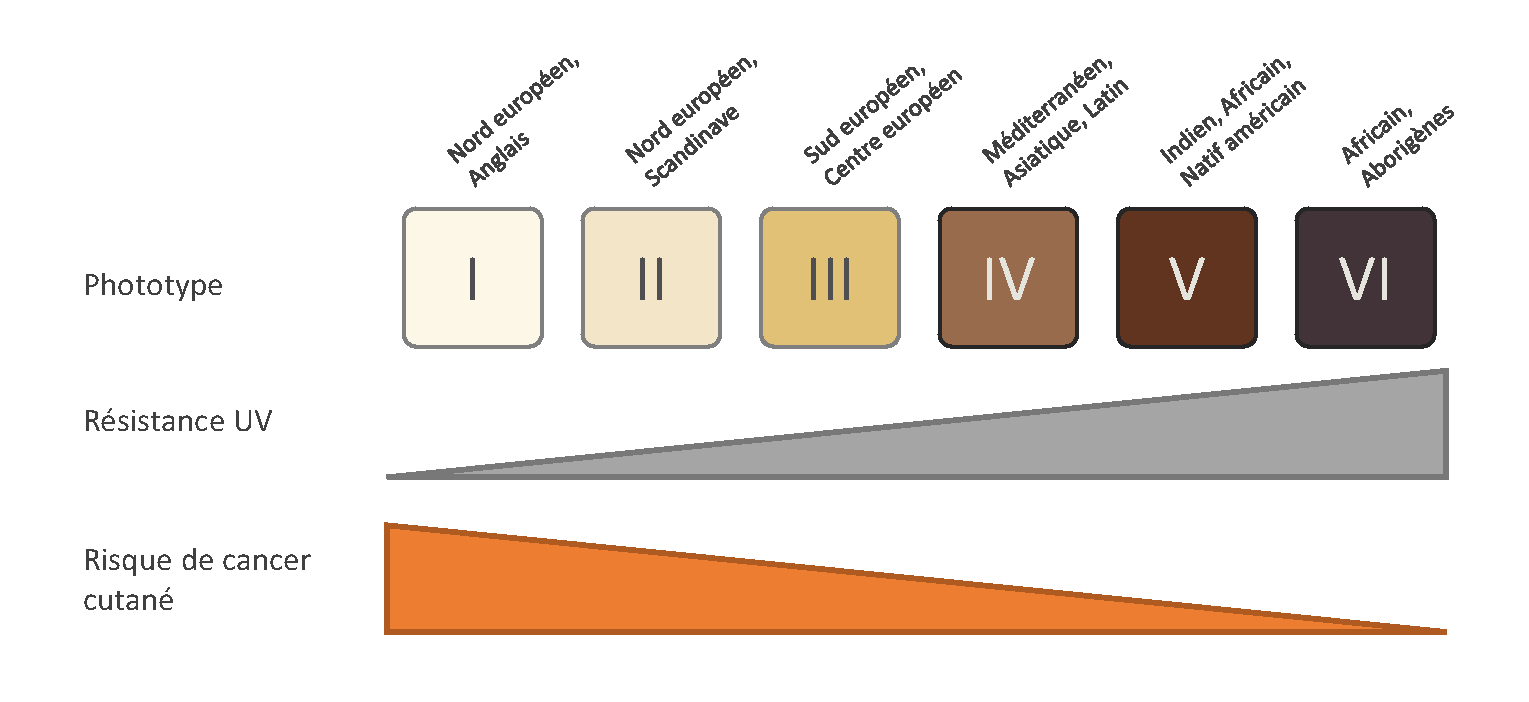
\includegraphics[width=\linewidth]{contents/chapter_1/resources/scheme_fitzpatrick_scale.pdf}
    \caption{Échelle de Fitzpatrick associant type de peau et caractéristiques associées \cite{Fitzpatrick1988}.}
    \label{fig:scheme_fitzpatrick_scale}
\end{figure}
Cet aspect est un élément important à prendre en compte lors de notre appréhension de la problématique. En effet, les travaux d'aide au diagnostic présent dans la littérature ne décrivent pas toujours les types de peau utilisés \cite{Celebi2007,Wiltgen2008,Koller2011}. Néanmoins, les échantillons présentés semble majoritairement axée sur les types I/II de peau, certaines pathologies seront ainsi plus enclin à une détection et/ou plus propices à certaines peaux \cite{Narayanan2010}. De plus, une même pathologie pourra diverger en terme de caractéristiques \cite{Tuma2015}. Nous retrouvons sur la \Cref{fig:scheme_fitzpatrick_scale}, une synthèse visuelle de ces types de peau et de leurs caractéristiques.

\section{Lésions de la peau}
Notre sujet abordant les lésions de la peau, il convient de définir le terme lésion pour bien situer l’objet de notre recherche. Selon PubMed, une lésion « correspond à toute anomalie touchant les tissus d’un organisme, généralement provoquée par une maladie ou par un traumatisme. » \textsuperscript{\ref{footnote:lesion_pubmed}}.\par
\addtocounter{footnote}{1}
\footnotetext[\thefootnote]{Source : Définition par \href{https://www.ncbi.nlm.nih.gov/pubmedhealth}{PubMed Health}. \label{footnote:lesion_pubmed}}

Les lésions de la peau correspondent à un terme générique caractérisant une partie de la peau ayant, en comparaison de la peau l’entourant, une croissance/apparence ou structure qui diffère. Ces lésions peuvent être pré ou post natal, comporter diverses formes et peuvent présenter différents risques.\par

Nous décrivons par le terme « lésion pigmentaire », les lésions affectant la peau présentant des pigmentations liées à la mélanine, au sang, ou de tout autre composant extérieur à la peau. Ces lésions peuvent être d’origine mélanocytaire (Nævus mélanocytaires) ou non mélanocytaire (nous nous intéresserons aux divers carcinomes lorsque nous aborderons les lésions malignes).\par

Nous traiterons sommairement des lésions de la peau au travers de ces quelques pages. Nous aborderons dans un premier temps les lésions bénignes et nous orienterons dans un second temps ce travail vers les lésions dites malignes. Enfin, nous présenterons le Lentigo, pathologie que nous étudierons dans ce manuscrit.\par

\subsection{Lésions bénignes}
Ces lésions désignent les diverses altérations classées comme sans gravité pour la santé. Néanmoins ces lésions peuvent présenter un terrain pour des lésions plus dangereuses.\par

L'une des lésions bénignes les plus communes est le naevus mélanocytaire souvent associé au « grain de beauté », à l’apparence de structures souvent circulaires ou ovales présentes en surface de peau chez l’homme. Les naevus sont susceptibles d’évoluer au cours du temps et peuvent dans très peu de cas aboutir à un mélanome. Ces tâches apparaissent durant les trente premières années de vie en moyenne et présentent des couleurs variées, avec des teintes allant du jaune vers le brun foncé. Voici quelques-unes des catégories et critères associés :
\begin{itemize}
\item Nævus commun, ou « grain de beauté » est le plus fréquent et se compose de mélanocytes regroupés en amas
\item Nævus atypique, se caractérise la plupart du temps par une pigmentation variable et des bordures irrégulières
\item Nævus congénital, apparaît en début de vie, peut apparaître sous forme de tâche
\item Nævus de Spitz, s’apparente souvent à un mélanome de part diverses caractéristiques. On y observe une croissance rapide en 2 à 6 mois ainsi qu’une couleur brun-rouge
\item Phénomène de Sutton, dé-pigmentation aux abords d’un naevus existant sur une durée de quelques semaines à quelques mois. Chez l’adulte, ce phénomène peut être un signe de mélanome.
\end{itemize}
Il convient de réaliser un surveillance régulière de ces lésions bénignes au sens large, afin de s'assurer qu'elles ne dégénèrent pas en pathologie maligne.\par

\subsection{Lésions malignes}
Avant de débuter, commençons par caractériser le terme malin, signifiant dans notre contexte « une maladie grave ou une tumeur pouvant se généraliser et entraîner la mort ». Nous traiterons au travers de cette partie des pathologies majeures, sujettes à entraîner le décès d’un individu. Ce décès est souvent la résultante de pathologie dites cancéreuses, c'est à dire « qui pour la plupart colonisent les tissus alentours, susceptibles de réapparaître après une tentative de retrait et de tuer le patient à moins d’être traitées de manière adéquate ».\par

Les cancers de la peau sont issus d’une division ou d’une mutation anormale de cellules de la peau et, résultent pour la plupart d’une exposition aux \gls{uv}, principal facteur de mutation. D’autres facteurs tels que le tabagisme, les virus, des prédispositions génétiques ou encore l’utilisation de médicaments immunosuppresseurs peuvent favoriser leur apparition. Les quelques sous parties suivantes donnent un aperçu des pathologies malignes majeures.\par

\subsubsection{Mélanome}
Le mélanome est une forme de cancer de la peau, se développant à partir de mélanocytes, également qualifié de tumeur mélanocytaire. Ce type de cancer se développe dans environ 70 \% des cas sur une peau saine et dans les 30 \% restants sur un naevus présent au préalable. Cette anomalie représente 2 \% des cas de cancers de la peau \cite{TortoraG;Derrickson2012}. Néanmoins, en contrepartie il s’agit de la forme la plus mortelle de cancer de la peau, avec au niveau mondial, une incidence de 350 000 cas en 2015. Ce cancer est par ailleurs responsable d’environ 59 800 décès \cite{Karimkhani2017}. Son incidence est fortement aggravée par l’exposition prolongée au soleil et plus particulièrement aux \gls{uv}. Les types I/II sur l’échelle de Fitzpatrick sont également les types de peau plus ciblés en proportion.\par

Comme pour les naevus, plusieurs types de mélanomes sont recensés, séparés en deux groupes distincts. D’une part les pathologies superficielles caractérisent les mélanomes présentant une phase d’extension épidermique (extension horizontale) suivi par une phase de développement en profondeur (extension verticale). Cette catégorie se compose de :
\begin{itemize}
\item Mélanomes d'extension superficielle – environ 70 \% des mélanomes
\item Mélanomes de Dubreuilh – environ 10 \% des mélanomes \cite{LeGal2011}
\item Mélanomes acro-lentigineux – environ 10 \% des mélanomes.
\end{itemize}
\begin{figure}[H]
    \centering
    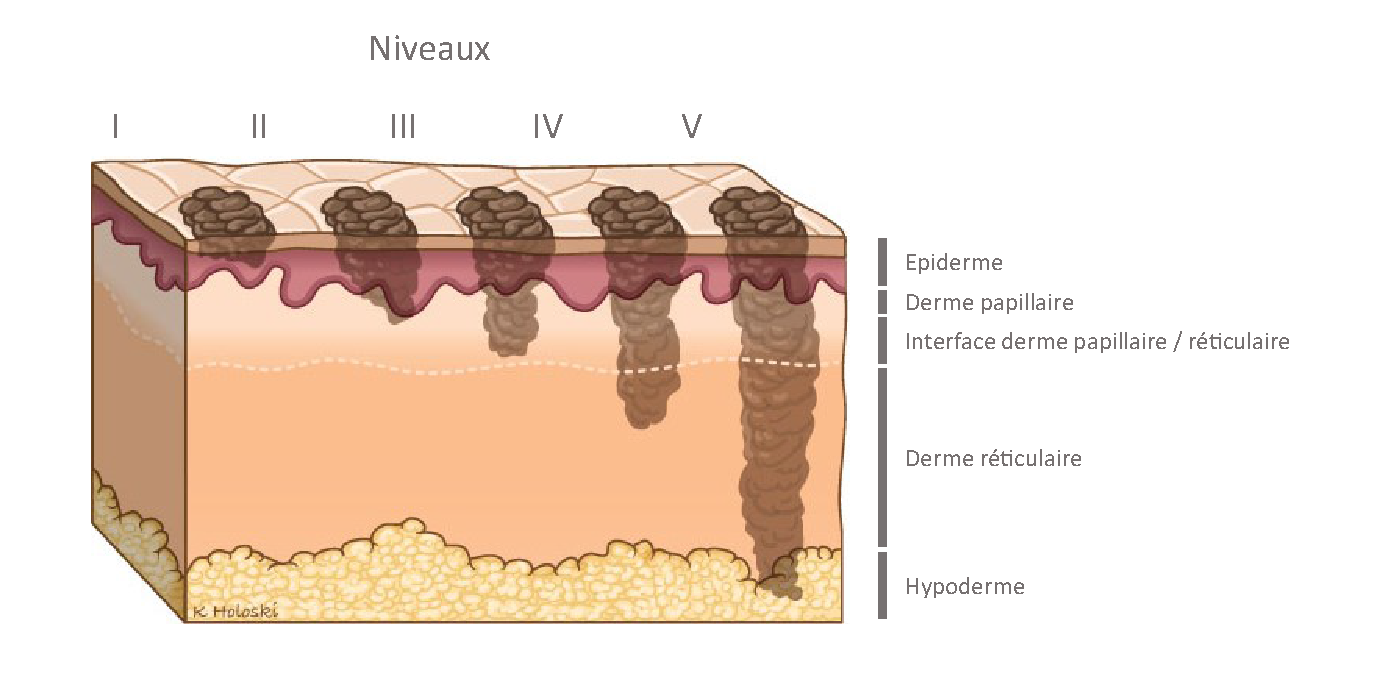
\includegraphics[width=0.7\linewidth]{contents/chapter_1/resources/illustration_clarklevels_kholoski.png}
    \caption{Illustration des différents niveaux de Clark \cite{Clark1969} \textsuperscript{\ref{footnote:illustration_clarklevels_kholoski}}.}
    \label{fig:illustration_clarklevels_kholoski}
\end{figure}\par

\addtocounter{footnote}{1}
\footnotetext[\thefootnote]{Image source : Dessin par \href{http://kholoski.com/}{Kellie Holoski} – Illustrateur médical. \label{footnote:illustration_clarklevels_kholoski}}
La seconde catégorie se compose des mélanomes nodulaires. Ceux-ci, se démarquent par une évolution plus rapide. En effet, dans une majeure partie, ceux-ci se développent verticalement dès les premiers symptômes. Une échelle, connue sous le nom de niveau de Clark (\Cref{fig:illustration_clarklevels_kholoski}), a été définie dans le but de caractériser le stade d’un mélanome \cite{Clark1969}.\par

\subsubsection{Carcinome spinocellulaire (ou épidermoïde)}
Les \gls{scc}, prennent racine au niveau des épithéliums de l’épiderme dont la croissance devient incontrôlée. L’apparence de cette pathologie est diverse, variant de simples plaques rouges à des cas de plaies ouvertes. Cette pathologie est plus à même de provoquer des métastases chez un individu, et donc de se propager.\par

Ce type de cancer est au second rang des cancers cutanés les plus graves, principalement lié à cette caractéristique de propagation. Ces cancers émergent le plus souvent de zones exposées régulièrement au soleil telles que le visage, les oreilles, le cou, etc… Ces zones exposées dénotent souvent de nombreux symptômes liés au dommage du soleil, comme :
\begin{itemize}
\item Des rides,
\item Une perte d’élasticité
\item Des tâches,
\item \ldots
\end{itemize}
Les prédispositions génétiques, les conditions de travail et le sexe d’un individu sont autant de facteur pouvant influer sur l’apparition de ce type de cancer.\par

\subsubsection{Carcinome basocellulaire}	
Le \gls{bcc} correspond à une surcroissance de cellules de l’épiderme, plus précisément de ses cellules basales. Il s’agit d’une des formes de cancer de la peau la plus commune, ses conséquences médicales sont par opposition moindres. En effet, ces cancers ont peu de risque de métastases et sont donc moins enclins à se propager à l’ensemble de l’organisme, et de provoquer la mort du patient. Ce cancer peut résulter de divers facteurs comme ses homologues, dont les principaux restent la surexposition au soleil ou la défaillance du système immunitaire.\par

\subsection{Une pathologie particulière : le Lentigo maligna}
\label{subsec:lentigo}
Le terme \gls{lm} et \gls{lmm} sont des alternatives anglo-saxonnes largement acceptées des termes francophones mélanome de Dubreuilh et mélanome sur mélanose de Dubreuilh qui touche les zones les plus exposées tel que le visage chez les populations âgées. Comme précédemment énoncé, ils représentent environ 10\% à 15\% des cas de mélanomes mais tendent à augmenter ces dernières années et vont désormais jusqu'à toucher les populations considérées comme jeunes. Le facteur le plus probable est l'exposition au soleil de plus en plus croissante chez ces différentes populations. Des études moléculaires et épidémiologiques tendent à distinguer deux principaux modes de développement de ces pathologies : l'une chez le sujet jeune, ayant de nombreux nævi et ayant une exposition solaire intermittente mais intense et l'autre chez le sujet plus âgé ayant été chroniquement exposé au soleil \cite{Baccard2009, LeGal2011, LeDuff2014}.\par

Le \gls{lm} est la résultante d'une prolifération de cellules au sein de la couche basale de l'épiderme, considérée par certains spécialistes comme melanoma-in-situ ou stade 0. Lorsque cette prolifération se propage aux couches inférieures par le biais des follicules pileux, nous parlons de \gls{lmm}. Le \gls{lm} est aussi souvent considéré comme un état pré cancéreux de la peau car ses cellules n'envahissent pas encore les régions profondes ou avoisinantes, et dont la croissance peut être très longue (jusqu'à 10 ans et plus). A l’œil nu, ces pathologies sont difficiles à distinguer de pathologies bénignes telles qu'un \gls{sl}, une \gls{sk} ou une \gls{pak} \cite{LeGal2011, LeDuff2014}. Des modèles de progression du stade ont été élaborés à partir d'observations comme en \cref{fig:illustration_surface_progression}.\par

\begin{figure}[H]
    \centering
    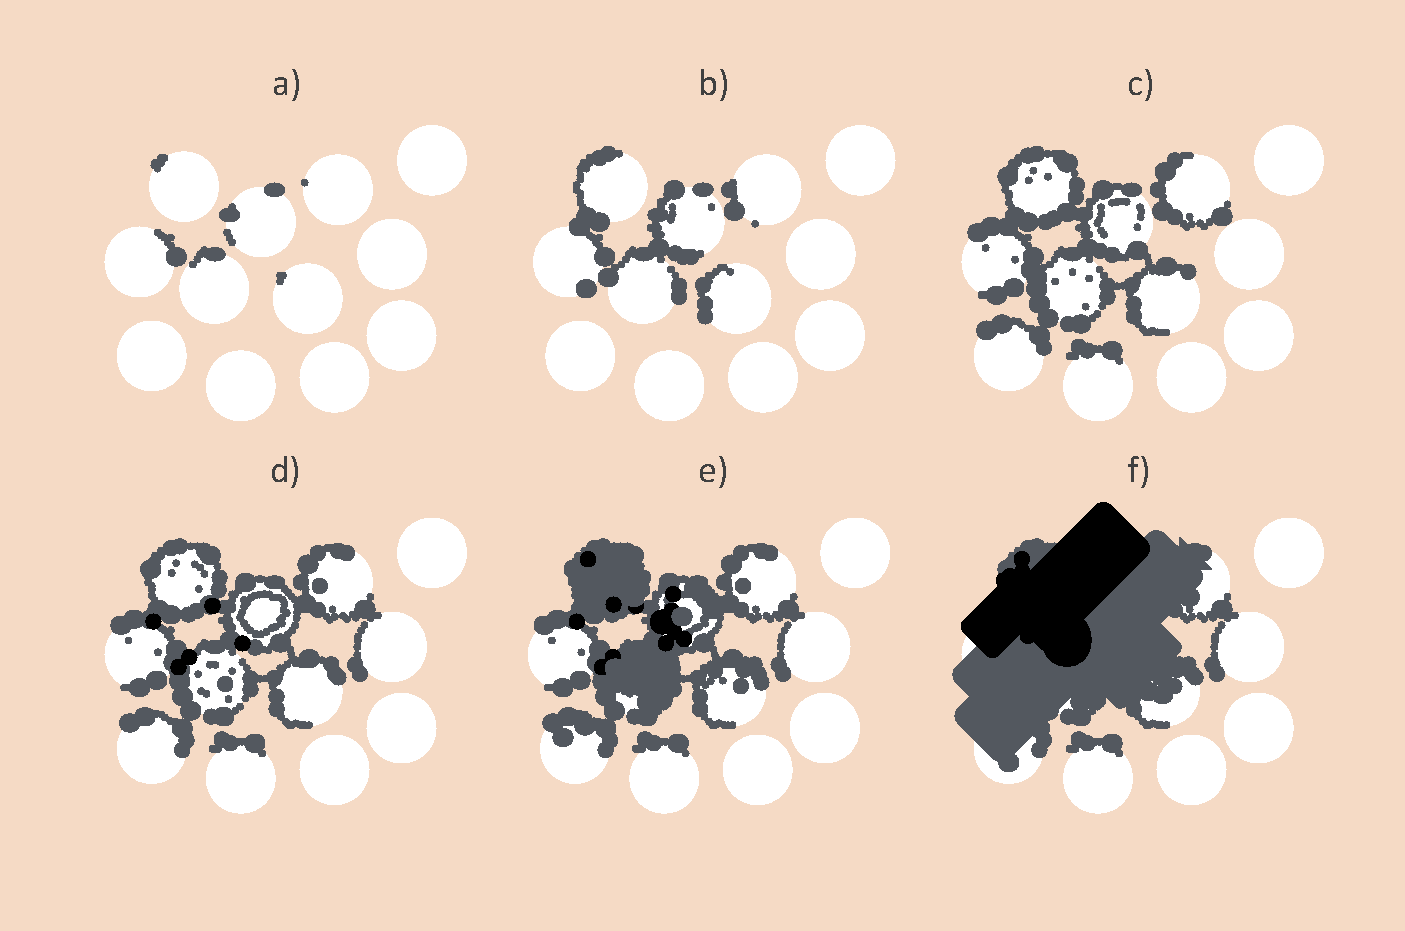
\includegraphics[width=0.8\linewidth]{contents/chapter_1/resources/illustration_surface_progression.jpg}
    \caption{Modèle de progression observée par dermatoscopie~\cite{Navarrete-Dechent2020}. En a), ce stade est marqué par une agglomération et une ouverture asymétriques en périphérie des follicules pileux ; en b), ce stade est marqué par l'apparition de nervures et de schémas granuleux ; en c), ce stade est marqué par l'apparition de structures rhomboïdales ; en d) ce stade est marqué par des zones homogènes et une oblitération des ouvertures folliculaires.}
    \label{fig:illustration_surface_progression}
\end{figure}\par

Le \gls{lm} et \gls{lmm} se caractérisent souvent par des macules pigmentées, des bordures et pigmentation irrégulières. Par ailleurs, ces pathologies touchent majoritairement les personnes de plus de 60 ans et des zones exposées telles que le visage ou le dos des mains.\par

En cas de doutes, ces lésions sont dans un premier temps abordées par un \textbf{diagnostic différentiel} lorsqu'il y a une ambiguïté : le médecin va observer l'ensemble des symptômes observables et environnementaux, puis va procéder par élimination des causes les plus fréquentes au causes les plus rares. Enfin, le médecin va confirmer son diagnostic si besoin par un \textbf{test de référence} (nous parlons souvent de "gold standard"), généralement celui de l'anatomopathologie, qui procédera :
\begin{inlinerate}
\item soit à une analyse histologique (discipline : histopathologie) c'est à dire une analyse structurelle du tissu,
\item soit à une analyse cythologique (discipline : cytopathologie) c'est à dire une analyse des cellules.
\end{inlinerate}
Dans les deux cas, le médecin procède à l'excision d'un tissu considéré comme pathologique (par biopsie), puis ce même tissu est préparé afin d'être observé par microscope. Ce type de procédure est relativement coûteux en temps, et représente une ressource financière importante si l'on considère le coût par patient. De plus, il s'agit d'une procédure incommodante pour le patient. De plus, une analyse peut échouer si le prélèvement est effectué en dehors de la zone pathologique \cite{LeGal2011}.\par

Les nombreuses contraintes actuelles liées aux coûts, à l'augmentation des patients et au respect du patient oriente vers des techniques non invasives plus rapides à mettre en oeuvre. Le chapitre suivant s'oriente en ce sens en apportant des bases quand aux propriétés phyisiques de la peau et à la manière de l'observer.\par

\begin{figure}[H]
    \centering
    \includegraphics[width=\linewidth]{contents/chapter_1/resources/example_lentigo_maligna.pdf}
    \caption{Exemple d'une pathologie de \gls{lm} perçue à l'aide de différents dispositifs médicaux. En a), un aperçu par photographie clinique ; en b), un aperçu par dermatoscopie ; en c), un aperçu par Microscopie confocale par réflectance. Les images d) et e), fournissent un aperçu par histologie.}
    \label{fig:example_lentigo_maligna}
\end{figure}\par